\documentclass[capchap,sumarioincompleto,a4paper,12pt,ruledheader,normaltoc]{utfprtex}%
\usepackage{polyglossia}
\setmainlanguage{portuges}
\usepackage[export]{adjustbox}
\usepackage{fontspec}
\setmainfont{Calibri}
\usepackage{utfprtexPropostaTCC}
\usepackage[brazil]{babel}
\usepackage[alf,abnt-emphasize=bf,abnt-etal-text=it,bibjustif,abnt-etal-cite=2,abnt-etal-list=0,abnt-full-initials=yes]{abntcite}
\usepackage{graphicx}
\usepackage{amsmath}
\usepackage{multirow}
\usepackage{pdflscape}
\usepackage{circuitikz}
\usepackage{multicol}
\usepackage{listings}
\usepackage{lscape}
\usepackage{tikz}
\usepackage[framed,numbered,autolinebreaks,useliterate]{mcode}
\renewcommand{\floatpagefraction}{0.90}
\renewcommand{\topfraction}{0.95}
\renewcommand{\bottomfraction}{0.95}
\renewcommand{\textfraction}{0.05}
\setlength{\intextsep}{5pt}
\setlength{\textfloatsep}{5pt}
\setlength{\floatsep}{5pt}

%---------- Autores ----------

\autorA{Callebe Soares Barbsoa}
\autorB{Rafael da Costa Bonotto}
\autorC{Raphael Henrique Soares Machado}
\autorD{Victor Emanuel Soares Barbosa}

%---------- Título ----------

\titulo{Relatórios, exercícios e fundamentação teórica relacionados a disciplina de Controle Digital}
\local{PATO BRANCO}
\data{2016}

\begin{document}

\capa
\newpage
\sumario
\newpage
\newpage

%---------- (Introdução)-------
\chapter{Introdução}

%---------- Primeira Prática  ----------
\chapter{Implementação da convolução}
\section{Objetivos}
 O objetivo principal desta prática é a implementação da convolução como ferramenta matemática para obtenção da saída de um sistema dada uma entrada qualquer e a resposta ao impulso.
 
\section{Fundamentação Teórica}
A convolução, pode-se assim dizer, é o equivalente entre sinais da multiplicação. Ela pode ser descrita em tempo contínuo, sendo chamada de integral de convolução e em tempo discreto de soma de convolução.

\subsection{Integral de convolução}
A resposta $y(t)$ a uma entrada $x(t)$ aplicada a um sistema T, sendo este linear e invariante no tempo, pode ser dado pela Equação \ref{Convolucao_continuo}, onde $h(t)$ é a resposta do sistema ao impulso. Esta dedução partiu da propriedade da função impulso dada na Equação \ref{definicao_delta}.

\begin{equation}
	x(t) = \int_{-\infty}^{\infty}x(\tau)\delta(t-\tau)d\tau
    \label{definicao_delta}
\end{equation}

\begin{eqnarray}
    y(t) &=& T{x(t)} \nonumber\\
    y(t) &=& T{\int_{-\infty}^{\infty} x(\tau)\delta {t-\tau}d\tau} \nonumber\\
    y(t) &=& \int_{-\infty}^{\infty} x(\tau)T{\delta {t-\tau}}d\tau \nonumber\\
    y(t) &=& \int_{-\infty}^{\infty} x(\tau)h{t-\tau}d\tau \nonumber\\
    y(t) &=& x(t)*h(t)
    \label{Convolucao_continuo}
\end{eqnarray}

\subsection{Soma de convolução}
A resposta em tempo discreto, $y[n]$, a uma entrada $x[t]$ aplicada a um sistema T, sendo este linear e invariante no tempo, pode ser dado pela Equação \ref{Convolucao_discreto}, onde $h[n]$ é a resposta do sistema ao impulso. Esta dedução partiu da propriedade da função impulso dada na Equação \ref{definicao_delta_discreto}.

\begin{equation}
	x[n] = \sum_{-\infty}^{\infty}x[k]\delta(n-k)
    \label{definicao_delta_discreto}
\end{equation}

\begin{eqnarray}
	y[n] &=& T{x[n]} \nonumber\\
	y[n] &=& T{\sum_{-\infty}^{\infty} x[k]\delta [n-]} \nonumber\\
    y[n] &=& \sum_{-\infty}^{\infty} x[k]T{\delta [n-k]} \nonumber\\
    y[n] &=& \sum_{-\infty}^{\infty} x[k]h[n-k] \nonumber\\
    y[n] &=& x[n]*h[n]
    \label{Convolucao_discreto}
\end{eqnarray}

\section{Procedimentos}
Foram resolvidos os exercícios 1 2 da apresentação de slides referente a transformada Z, com código implementado em Matlab.

\subsection{Exercício 1}
Determine a saída do sistema com
resposta ao impulso h[n] e para um sinal de entrada
x[n], ambos sinais estão mostrados na Figura \ref{fig:procedimento_pr1_ex1}:\\
A) análise gráfica por impulsos \\
B) cálculo/tabela de convolução \\
C) convolução utilizando ferramenta
computacional: \emph{script} Matlab

\begin{figure}[!th]
	\centering
    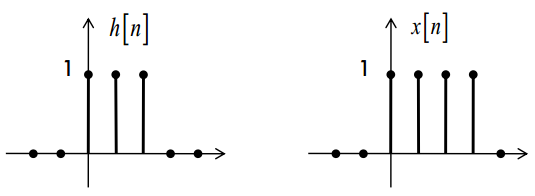
\includegraphics[scale = .7]{Imagens/Execicio1.PNG}
    \caption{Sinais do Exercício 1, prática 1.}
 \label{fig:procedimento_pr1_ex1}
\end{figure}

\subsection{Exercício 2}
Considere um sistema que possui resposta
ao impulso h[n]=$2^{-nT}$ e o sinal de entrada é uma onda
retangular (razão cíclica 40\%, D=0,4) com período
10s e amplitude 3,3V.\\
A) Determine a resposta (sinal de saída) do sistema para
3 períodos do sinal de entrada considerando que o
periodo de amostragem é T=0.2s.\\
B) Considere um ruído de 10\% no sinal de entrada e
repita o item A.\\
C) Considere um sinal de entrada senoidal com mesmo
período, amplitude e ruído dados acima.

\section{Resultados e discussões}

\subsection{Exercício 1}
\subsubsection{C)}
O código implementado em Matlab para a resolução da letra C do exercício 1 está logo abaixo:
\lstinputlisting{Arquivos_tex/Aula_3_Exercicio_1.m}

Obtendo como saída o gráfico da Figura \ref{saida_ex1_pr_1}

\begin{figure}
	\centering
    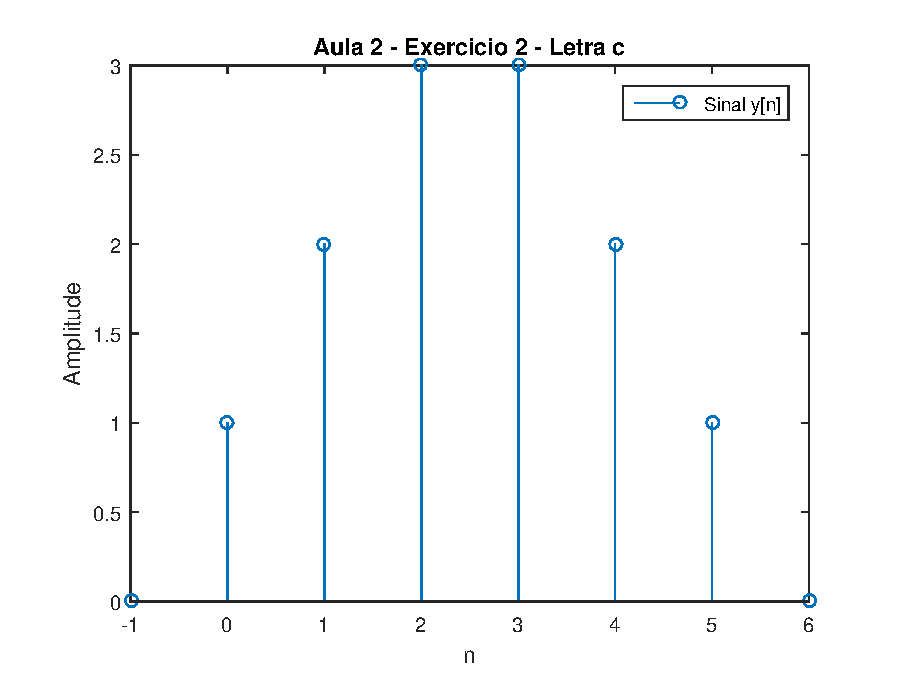
\includegraphics[scale = .7]{Imagens/Aula_3_exercicio1_LetraC.eps}
    \caption{Gráfico de saída do código do Exercício 1, letra C, prática 1.}
    \label{saida_ex1_pr_1}
\end{figure}

\subsection{Exercício 2}
O código implementado em Matlab para a resolução do exercício 2 está logo abaixo:
\lstinputlisting{Arquivos_tex/Aula_3_Exercicio_2.m}

Obtendo como saída os gráfico das Figuras \ref{saida_ex2_pr_1_L_A}, \ref{saida_ex2_pr_1_L_B} e \ref{saida_ex2_pr_1_L_C}.

\begin{figure}[!ht]
	\centering
    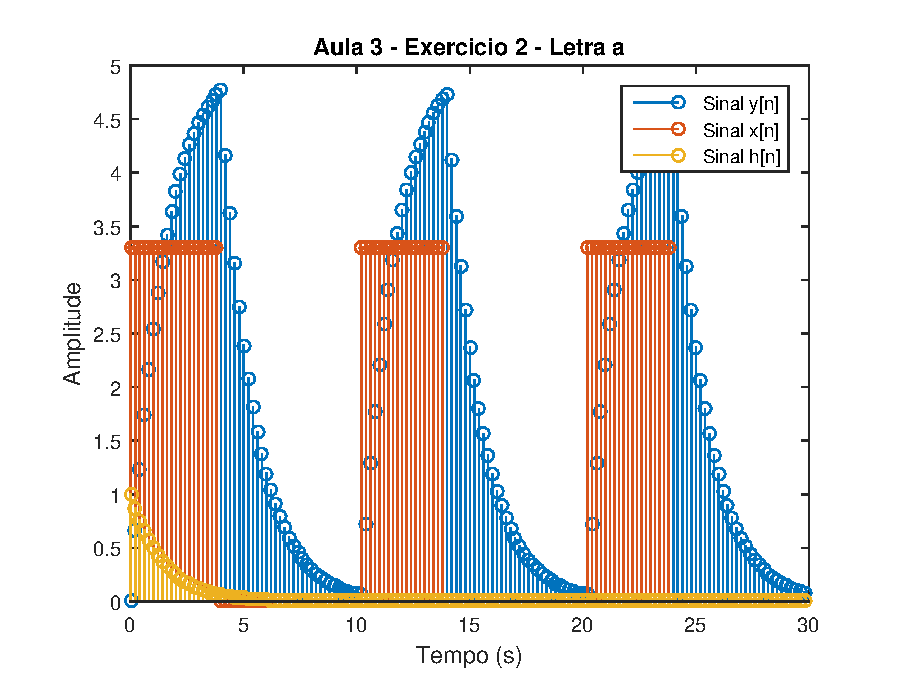
\includegraphics[scale = 1]{Imagens/Aula_3_exercicio2_LetraA.eps}
    \caption{Gráfico de saída do código do Exercício 2, letra A, prática 1.}
    \label{saida_ex2_pr_1_L_A}
\end{figure}

\begin{figure}[!ht]
	\centering
    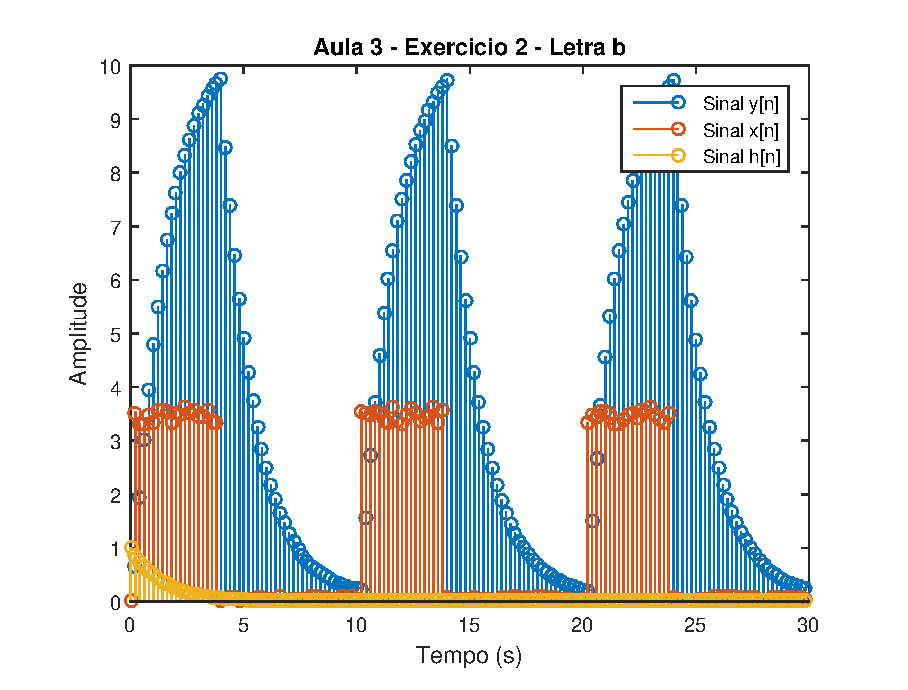
\includegraphics[scale = 1]{Imagens/Aula_3_exercicio2_LetraB.eps}
    \caption{Gráfico de saída do código do Exercício 2, letra B, prática 1.}
    \label{saida_ex2_pr_1_L_B}
\end{figure}

\begin{figure}[!ht]
	\centering
    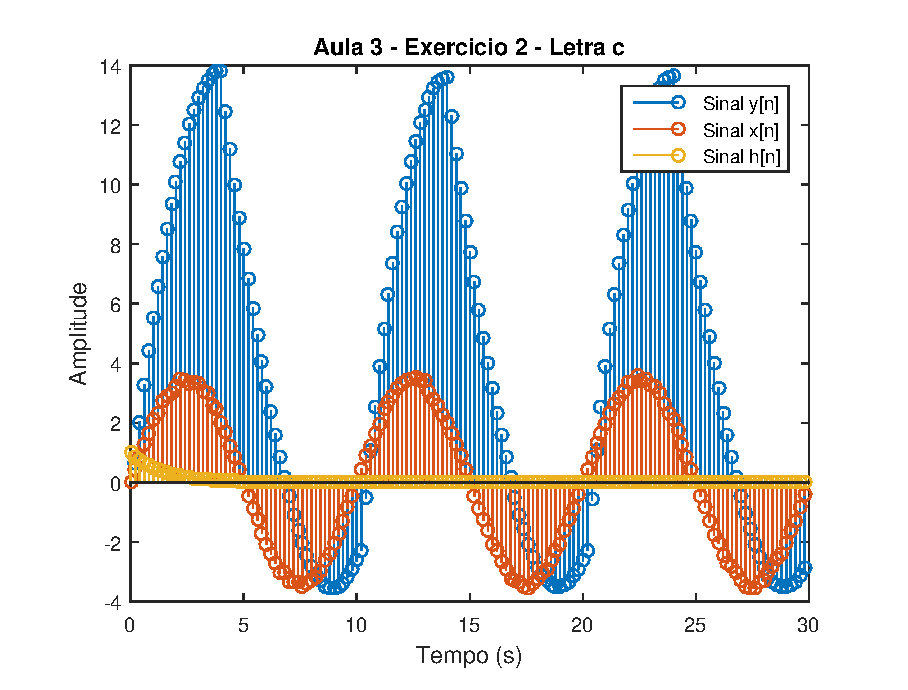
\includegraphics[scale = 1]{Imagens/Aula_3_exercicio2_LetraC.eps}
    \caption{Gráfico de saída do código do Exercício 2, letra C, prática 1.}
    \label{saida_ex2_pr_1_L_C}
\end{figure}

\textcolor{red}{COMENTAR E DISCUTIR RESULTADOS}

%---------- Segunda Prática  ----------
\chapter{Simulação de um sistema discreto com equações diferenças}
\section{Objetivos}
 O objetivo principal desta prática é a simulação em Matlab de um sistema de controle digital completo dado as equações em Z que descrevem os blocos constituintes do sistema em malha fechada.

\section{Fundamentação Teórica}
Para realização desta prática se utilizou a teoria da transformada Z inversa, em específico o método das equações de diferenças. Este método é facilmente utilizado e computadores digitais por fornecer a equação em tempo discreto da transforma inversa de \textit{z} .

Quando obtemos a transformada inversa de \textit{z}, assumimos que a sequência $x(kT)$ ou $x(k)$ é zero para $k<0$. Nota-se que em aplicação de engenharia de controle e processamento de sinais, $X(z)$ é frequentemente expressado com a razão polinomial de $z^{-1 }$, como apresentado na equação (\ref{pr_2_1})
\begin{equation}
G(z) = \frac{Y(z)}{X(z)} = \frac{b_0z^{-(n-m)}+b_1z^{-(n-m+1)}+...+ b_mz^{-n}}{1 + a_1z^{-1} + a_2z^{-2} + ... + a_nz^{-n}} \ \   (m \leq n)
	\label{pr_2_1}
\end{equation} 
Pelo método aproximado de equações de diferenças convertemos a equação (\ref{pr_2_1}) para a equação (\ref{pr_2_2}),
$$
(1 + a_1z^{-1} + a_2z^{-2} + ... + a_nz^{-n})Y(z) = (b_0z^{-(n-m)}+b_1z^{-(n-m+1)}+...+ b_mz^{-n})X(z) 
$$
\begin{eqnarray}
y(k) + a_1y(k-1) + a_2y(k-2) + ... + a_ny(k-n) =  b_0x(k-(n-m)) + ... \nonumber \\ 
... b_1x(k-(n-m+1)) + ... + b_mx(k-n) \nonumber \\
y(k) = - a_1y(k-1) - a_2y(k-2) + ... + - a_ny(k-n) + b_0x(k-(n-m)) + ... \nonumber \\ 
... b_1x(k-(n-m+1)) + ... + b_mx(k-n)
\label{pr_2_2}
\end{eqnarray}

Achando a transformada inversa \textit{z} de $Y(z)$, resolve-se a equação de diferença $y(k)$ facilmente por linguagem de programação.


\section{Procedimentos}
O exercício consistiu em simular um sistema de tempo discreto para período de amostragem de 0,1 s para sinal de entrada uma onda quadrada de amplitude 0 - 5 V, com período de 10s e 2\% de ruído randômico. O sistema está mostrado na Figura \ref{fig:pr2_esquema}, bem como as equações dos blocos estão descritas abaixo:

\begin{equation}
C(z) = 0,9*\frac{z-0,8}{z-1}
\label{pr_2_C}
\end{equation}

\begin{equation}
	G(z) = \frac{0,3z}{(z-0,5)(z-0,2)}
    \label{pr_2_G}
\end{equation}

\begin{equation}
	S(z) = \frac{0,2}{z-0,8}
    \label{pr_2_S}
\end{equation}

\begin{figure}[!th]
	\centering
    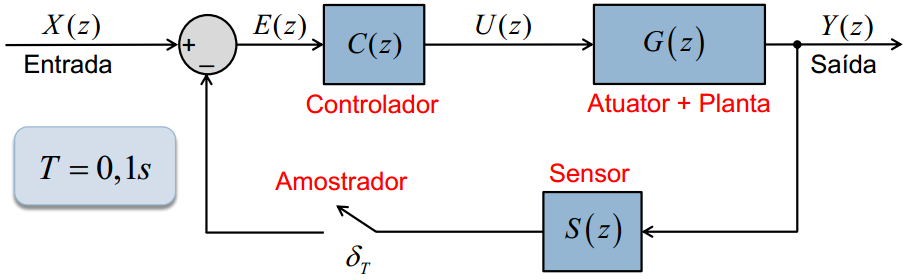
\includegraphics[scale = .5]{Imagens/Execicio1_pr2.PNG}
    \caption{Diagrama de blocos da prática 2.}
    \label{fig:pr2_esquema}
\end{figure}

\section{Resultados e discussões}

Realizando o equacionamento genérico a malha fechada do sistema apresentado na Figura \ref{fig:pr2_esquema} encontra-se a equação (\ref{pr_2_3})  
\begin{equation}
\frac{Y(z)}{X(z)} = \frac{C(z)G(z)}{1 + C(z)G(z)S(z)}
\label{pr_2_3}
\end{equation}

Substituindo as equações (\ref{pr_2_C}), (\ref{pr_2_G}) e (\ref{pr_2_S}) na equação (\ref{pr_2_3}) e expressado com a razão polinomial de $z^{-1 }$ temos

\begin{equation}
\frac{Y(z)}{X(z)} = \frac{0,27z^{-1} - 0,216z^{-2}}{1 - 1,7z^{-1} + 0,854z^{-2} - 0,1z^{-3}}
\label{pr_2_4}
\end{equation}

Através da equação (\ref{pr_2_4}) aplica-se o método da equação de diferença conforme apresentado na equação (\ref{pr_2_2}), concebendo a equação (\ref{pr_2_5}) que será simulada com o respectivo sinal de entrada.

\begin{equation}
y(k) =  1,7y(k-1) - 0,854y(k-2) + 0,1y(k-3) + 0,27x(k-1) - 0,216x(k-2)
\label{pr_2_5}
\end{equation}

O código implementado em Matlab está mostrado abaixo:
\lstinputlisting{Arquivos_tex/Aula_5_Exercicio_2.m}

Obtendo como saída o gráfico da Figura \ref{saida_ex2_pr_2}.

\begin{landscape}
  \begin{figure}[!ht]
      \centering
      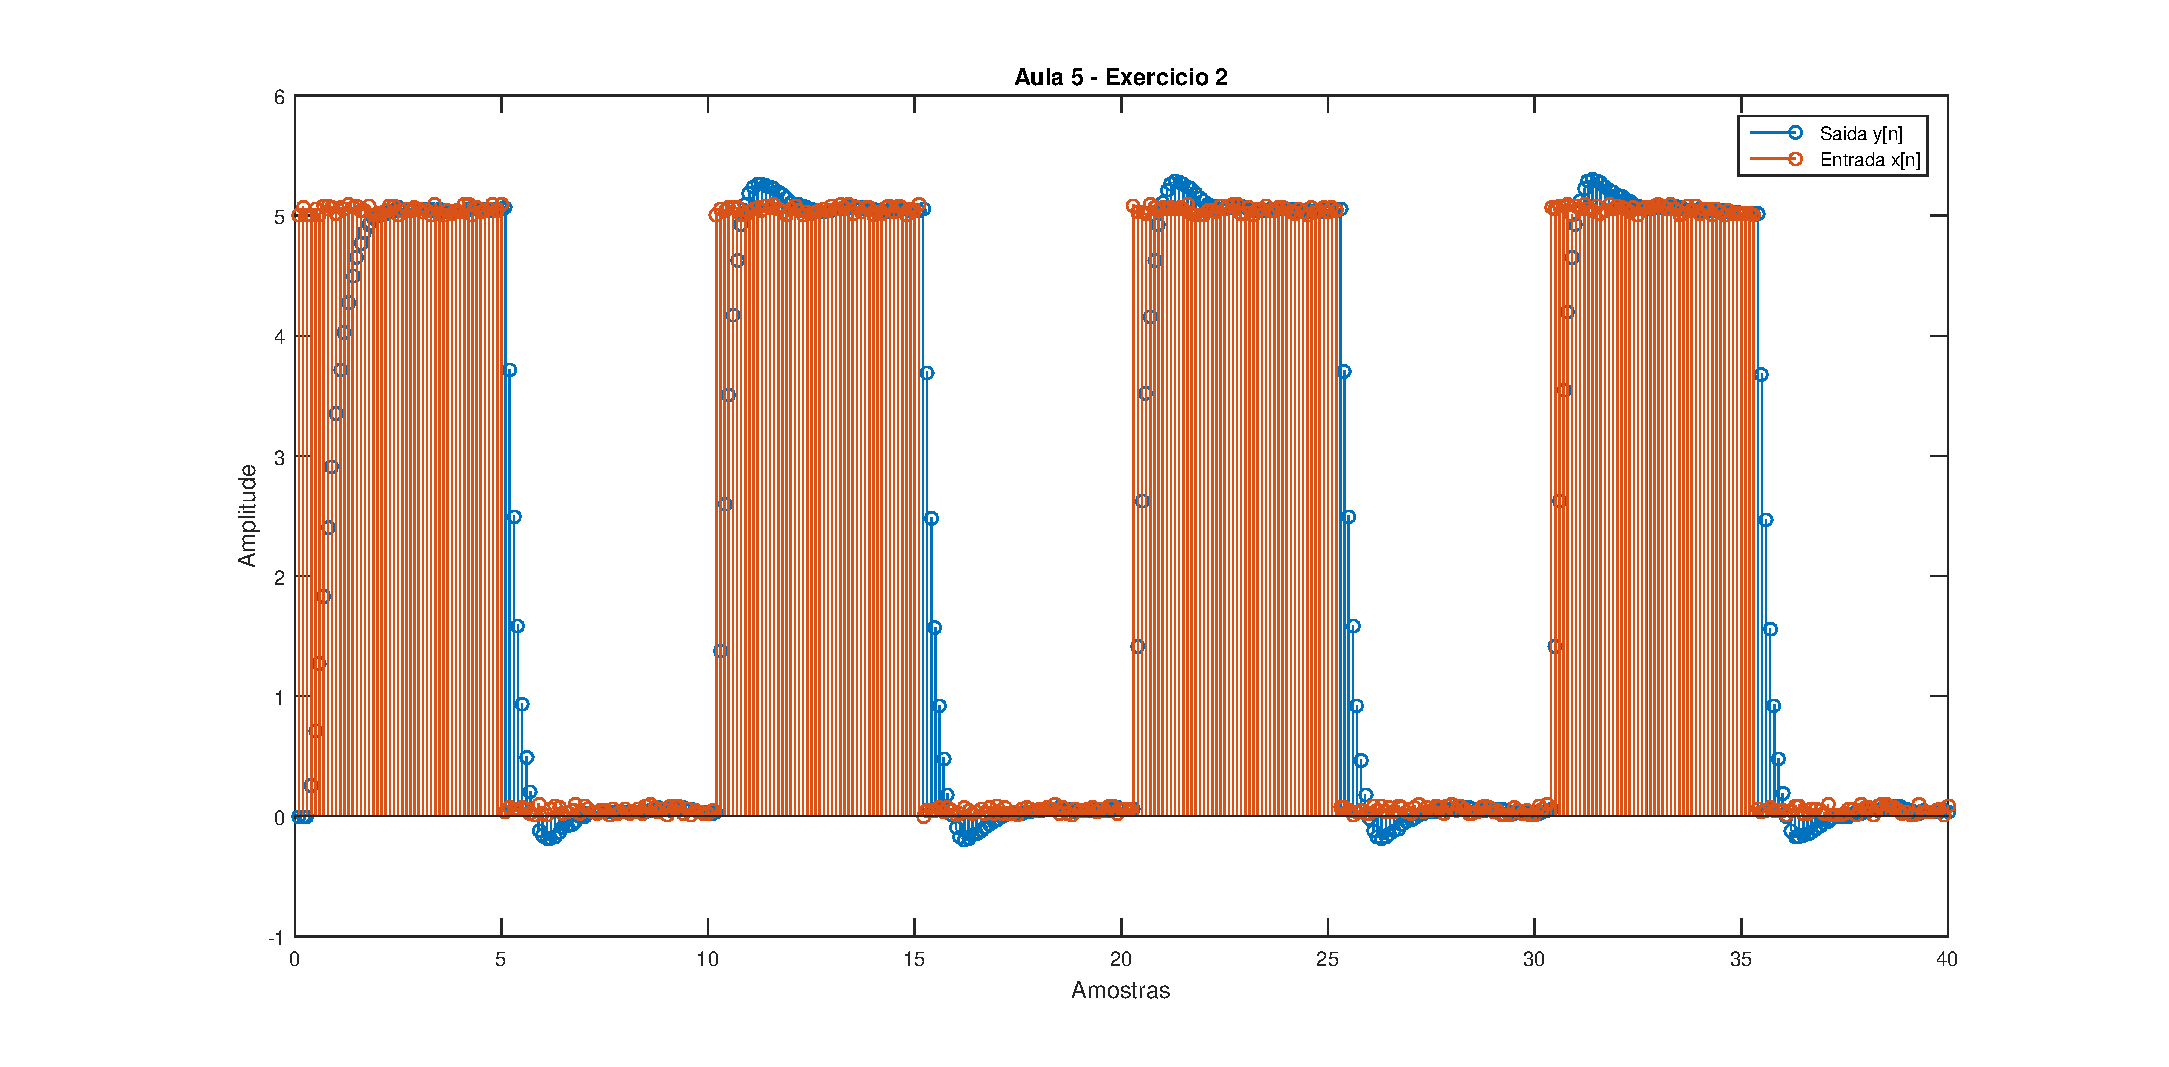
\includegraphics[scale = .66]{Imagens/Aula_5_exercicio2.eps}
      \caption{Gráfico de saída do código do exercício da prática 2.}
      \label{saida_ex2_pr_2}
  \end{figure}
\end{landscape}

A transformada $z$ é uma ferramenta comumente utilizada para análise e síntese de sistemas de controle em tempo discreto. Análoga a transformada de Laplace, possui a equação de diferenças como ferramenta matemática para a obtenção da resposta do sistema a uma dada entrada. 

Como a natureza exprime sistemas variáveis no tempo de forma contínua, a transformada inversa $z$ permitiu através do método de equações de diferenças fornece a saída em tempo discreto fazendo uso do tempo de amostragem que simule um sistema pseudo-contínuo.

Este método recursivo possibilitou a implementação digital, conforme o exercício apresentado, de forma simplista utilizando laço de controle e vetores. Na Figura \ref{saida_ex2_pr_2}, dado a entrada de uma onda quadrada, o PID, a planta e o sensor interagem na malha fornecendo uma resposta com baixo sobresinal e rápido tempo de assentamento.

%---------- Terceira Prática  ----------
\chapter{Modulador PWM e Sist.Cond. Sinais e ADC}
\section{Objetivos}

\section{Fundamentação Teórica}

\section{Procedimentos}

\section{Resultados e discursões}

%---------- Quarta Prática  ----------
\chapter{Amostragem de sinais e análise em Frequência de sinais Amostrados}
\section{Objetivos}
Nesta prática objetiva-se apresentar os princípios elementares para amostragem de sinais
\section{Fundamentação Teórica}

Sendo o sinal analógico contínuo no tempo e amplitude, contém uma infinidade de valores. O aparelhos de processamento digital possuem uma banda passante limitada, acarretando na finitude de amostras utilizada para formação do sinal. 

A amostragem de um sinal analógico é caracterizada como o processo pelo qual o mesmo é representado por um conjunto discreto de números. Este número, ou amostras, são iguais ao valor no sinal neste respectivo instante. A quantidade de amostras é definida pela frequência de amostragem (frequência de coleta dos valores) comparado a frequência fundamental do sinal.

A escolha da frequência de amostragem é baseado no \textit{Teorema de amostragem de Nyquist e Shannon}. Este teorema basicamente estabelece que o sinal é precisamente  reconstruído por amostras sob a condição que componente de maior frequência não deve ser maior que metade da taxa de amostragem.

Quando este teorema não é obedecido, ocorre \textit{folding} e/ou \textit{aliasing}, fenômeno de sobreposição do espectro de frequência conhecido. Um filtro anti-\textit{aliasing }analógico é frequentemente colocado entre o sensor e o conversor A/D tendo como função, a redução das componentes de ruídos em alta frequência
\section{Procedimentos}
O exercício consistiu em utilizar o $Simulink^{\textregistered}$ para a construção do sinal contínuo no tempos com as seguintes  componentes frequências:

\begin{itemize}
	\item $f_0$ = 1 Hz;
	\item $f_1$ = 5 Hz;
	\item $f_2$ = 100 Hz; 
\end{itemize}

Sendo estes sinais amostrados  por um filtro \textit{Zero-order-hold} (ZOH) com as seguintes frequências de amostragem ($f_s$):

\begin{itemize}
	\item $f_{s1}$ = 10 Hz;
	\item $f_{s2}$ = 100 Hz;
	\item $f_{s3}$ = 1000 Hz; 
\end{itemize}

Na análise do espectro foi utilizado o comando FFT do $Matlab^{\textregistered}$, de forma a verificar o fenômeno de \textit{aliasing}	 para cada caso da frequência de amostragem. Para as frequências onde ocorreram  foi projeto um filtro passa-baixa.


\section{Resultados e discursões}

\begin{figure}[!th]
	\centering
	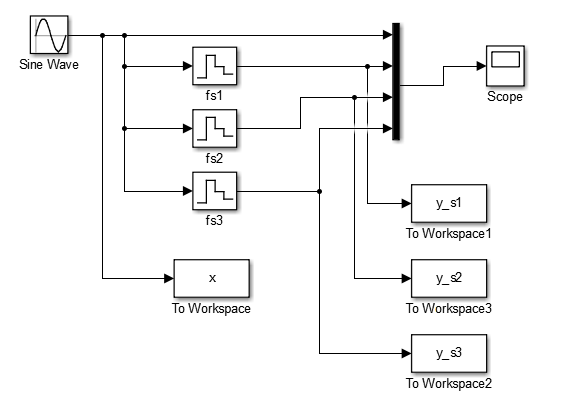
\includegraphics[scale = .55]{Imagens/pratica4_1.PNG}
	\caption{Diagrama de blocos da prática 4.}
	\label{fig:pr4_esquema}
\end{figure}

\begin{figure}[!th]
	\centering
	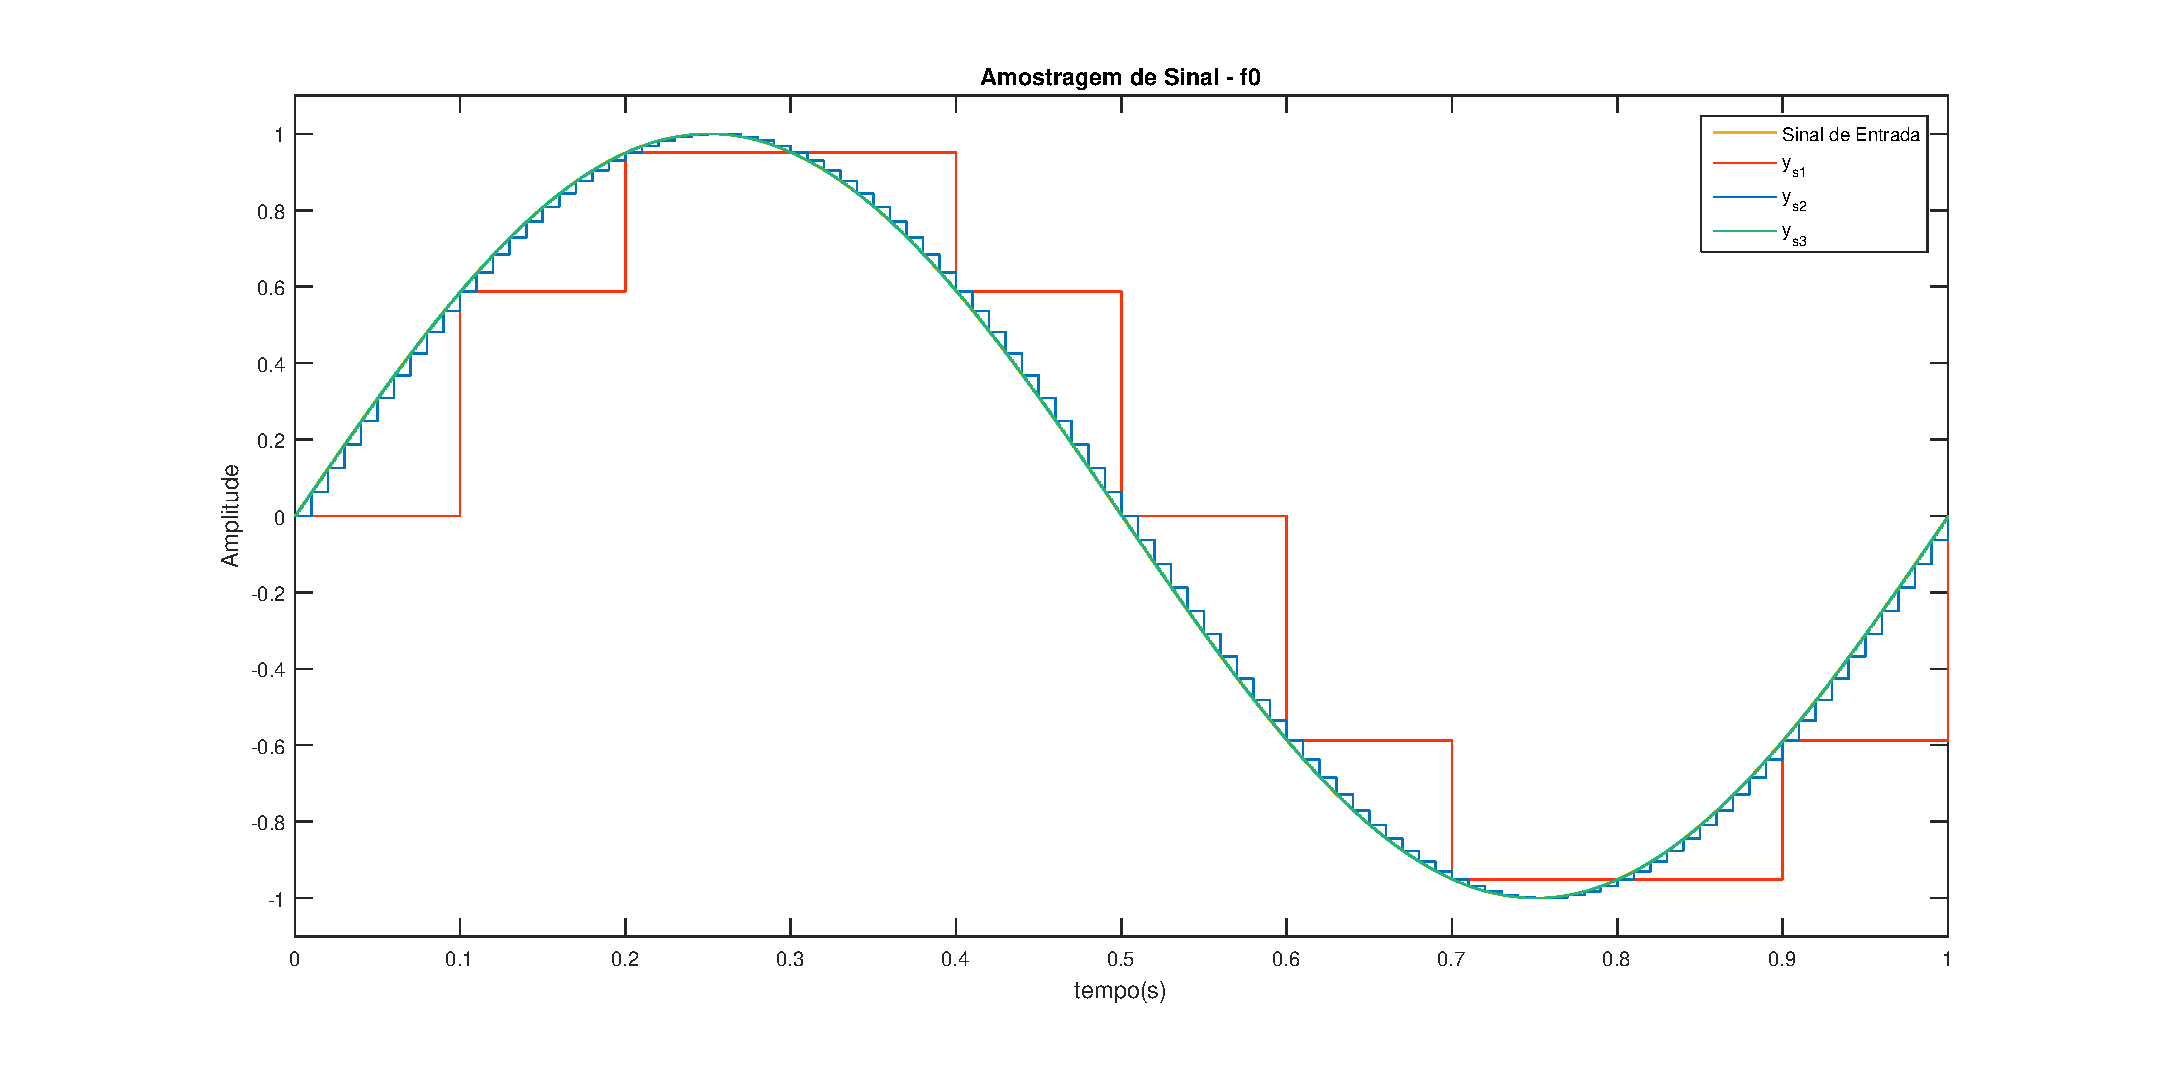
\includegraphics[scale = .45]{Imagens/pratica4_2.eps}
	\caption{Diagrama de blocos da prática 4.}
	\label{fig:pr4_esquema}
\end{figure}

\begin{figure}[!th]
	\centering
	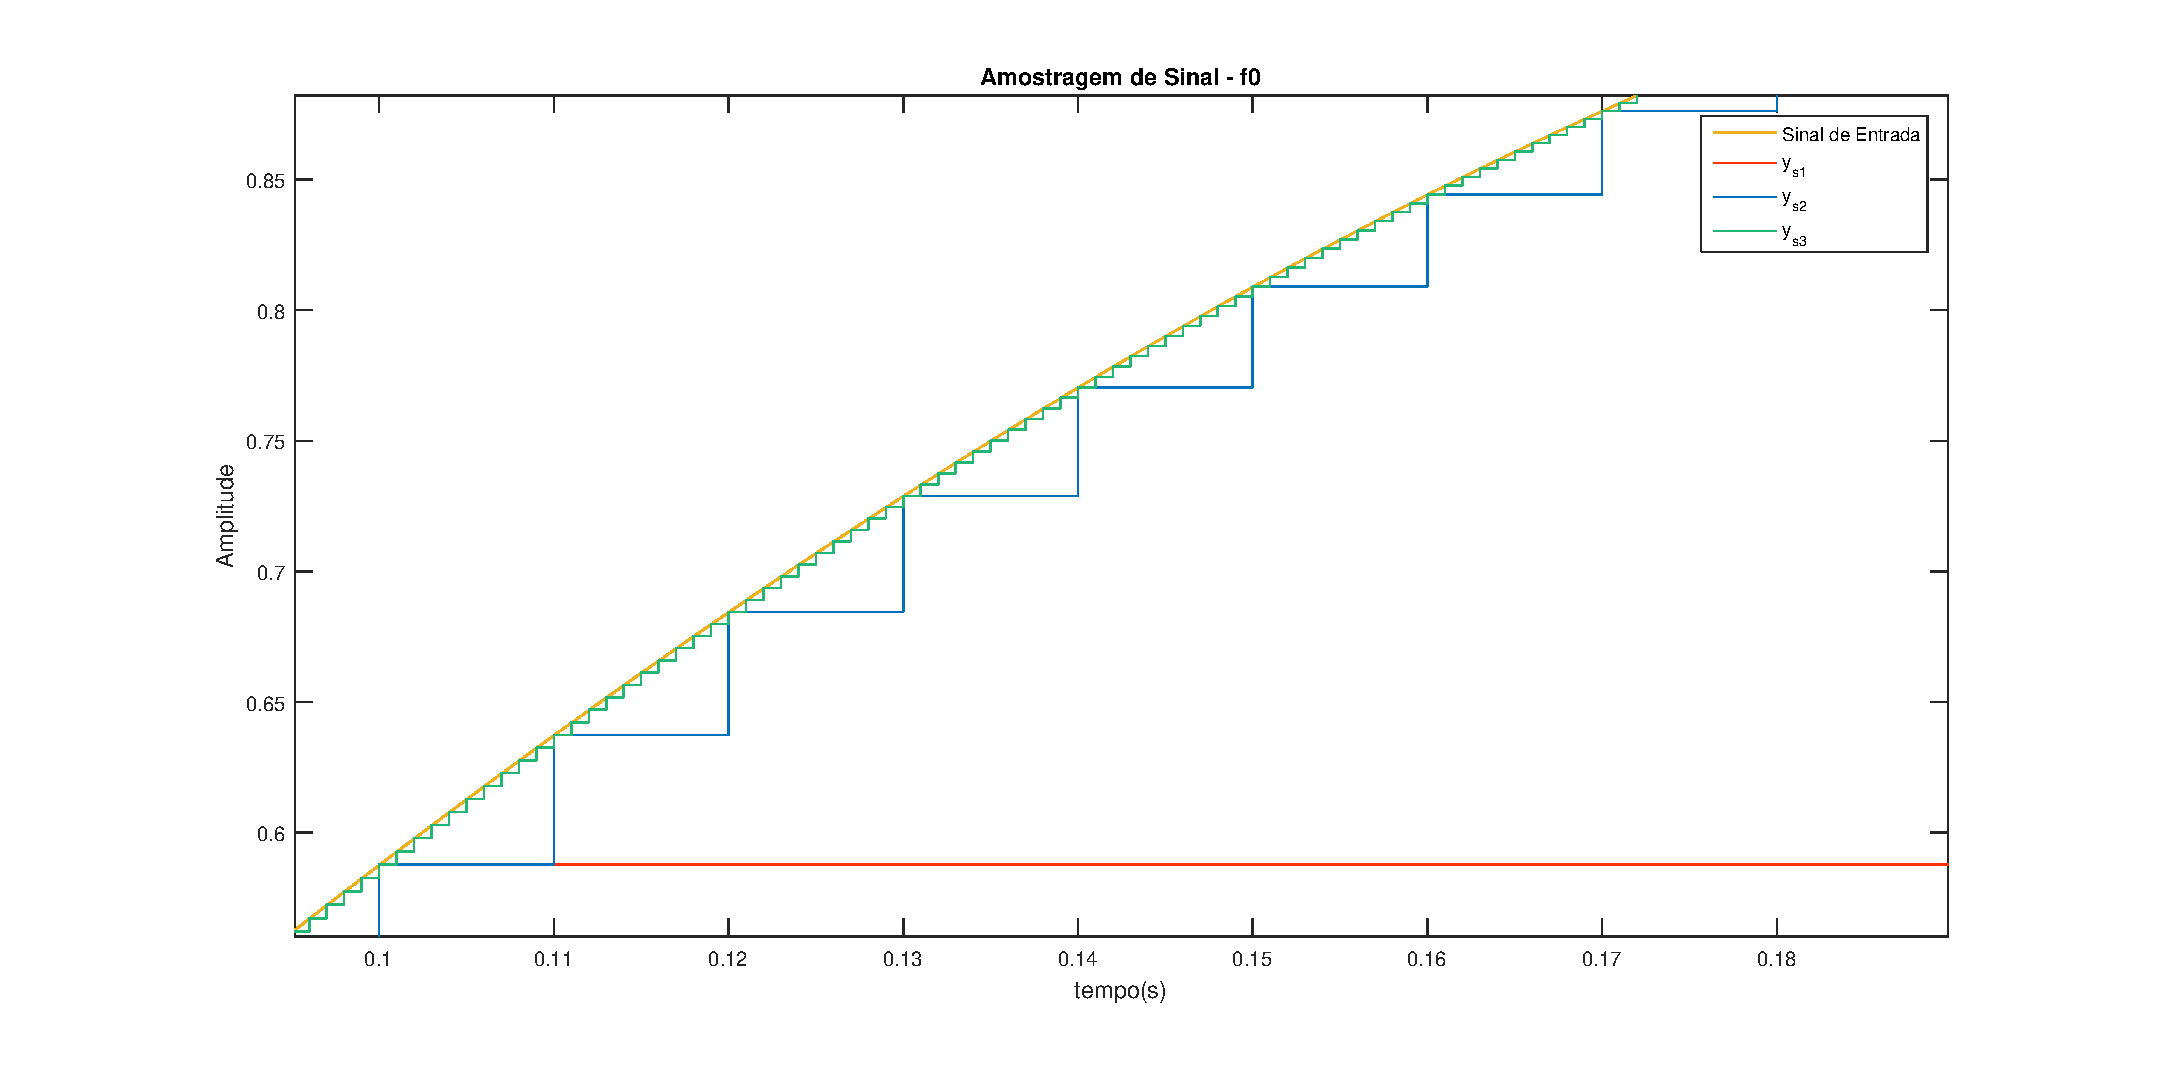
\includegraphics[scale = .45]{Imagens/pratica4_3.eps}
	\caption{Diagrama de blocos da prática 4.}
	\label{fig:pr4_esquema}
	\end{figure}
	
	\begin{figure}[!th]
		\centering
		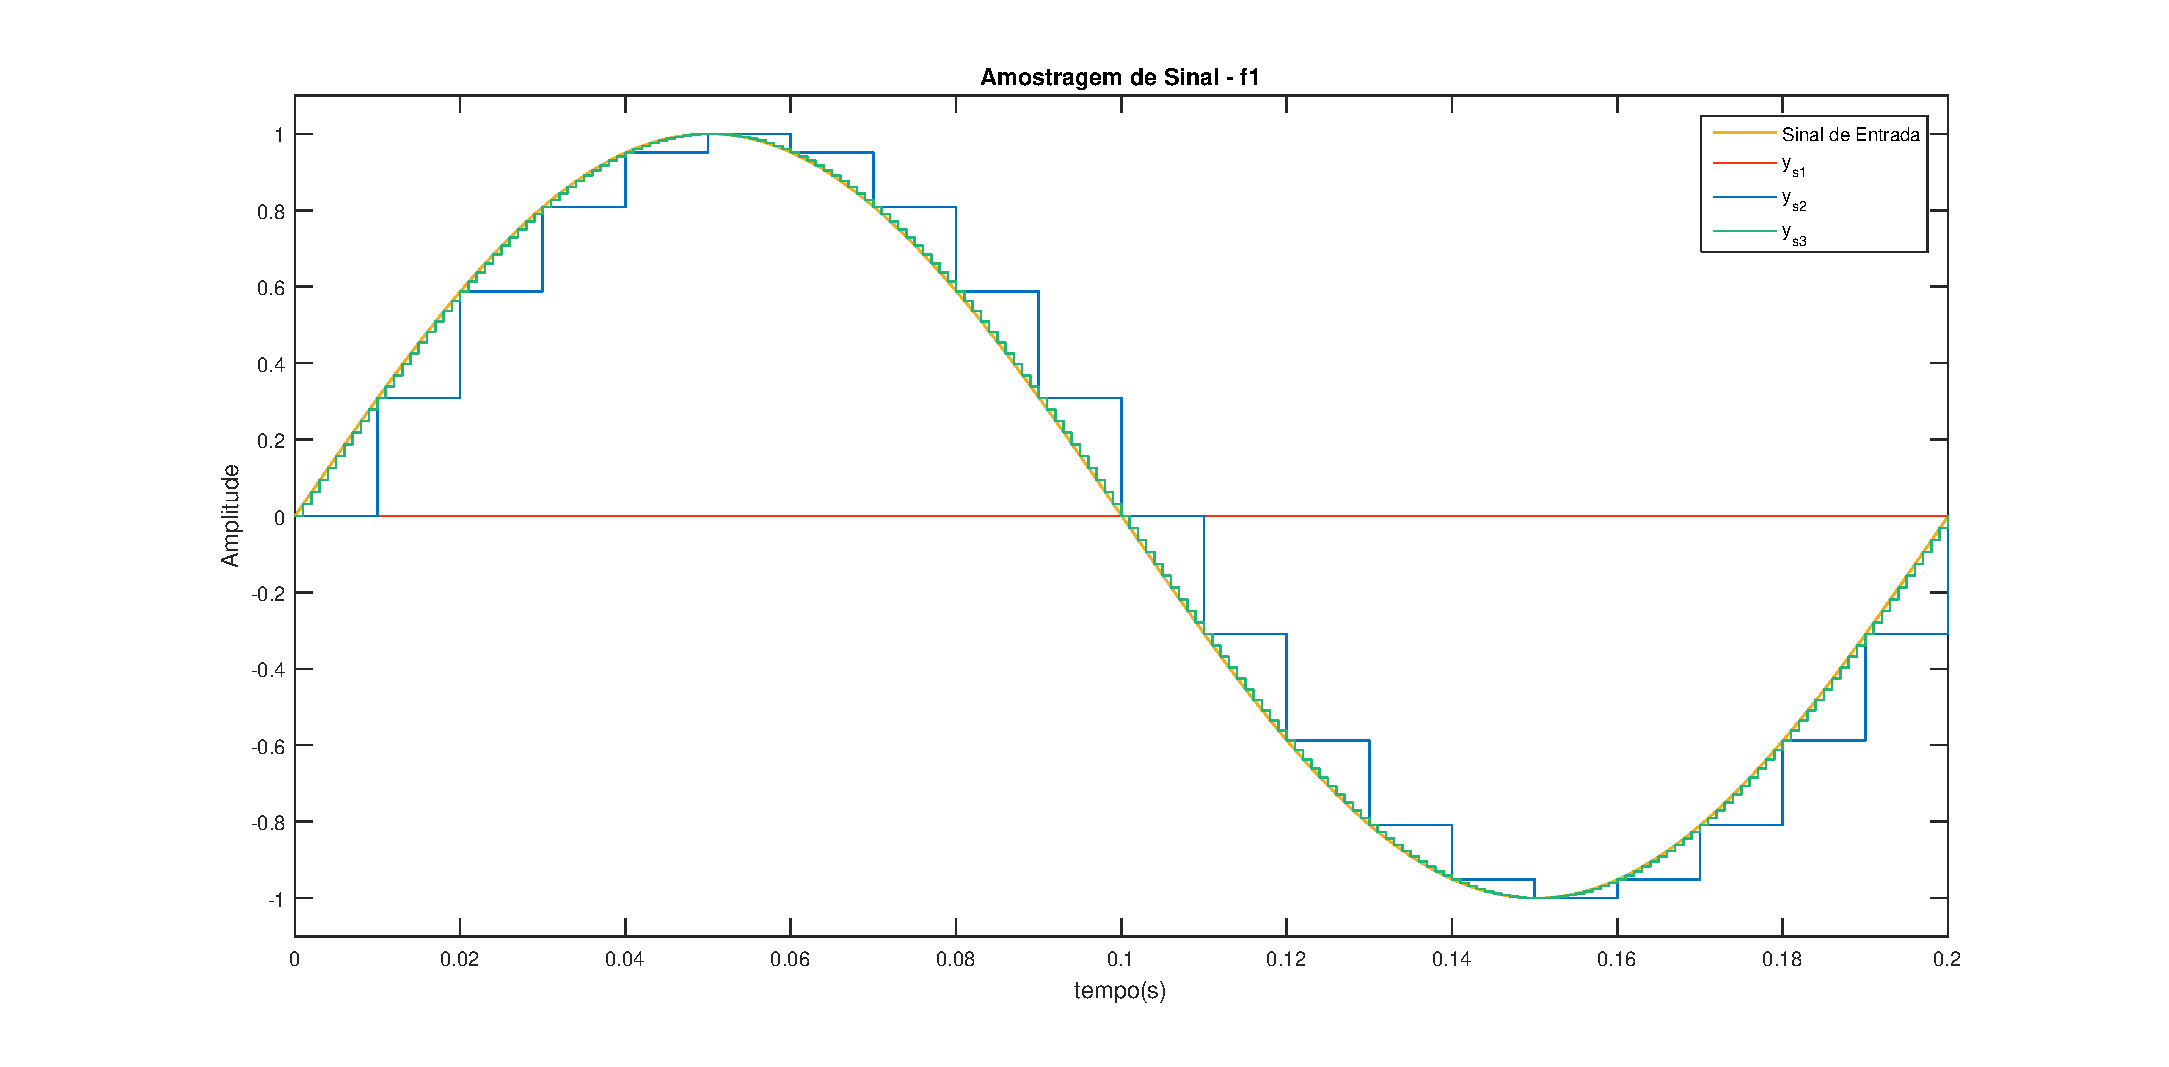
\includegraphics[scale = .45]{Imagens/pratica4_4.eps}
		\caption{Diagrama de blocos da prática 4.}
		\label{fig:pr4_esquema}
		\end{figure}
		
\begin{figure}[!th]
	\centering
	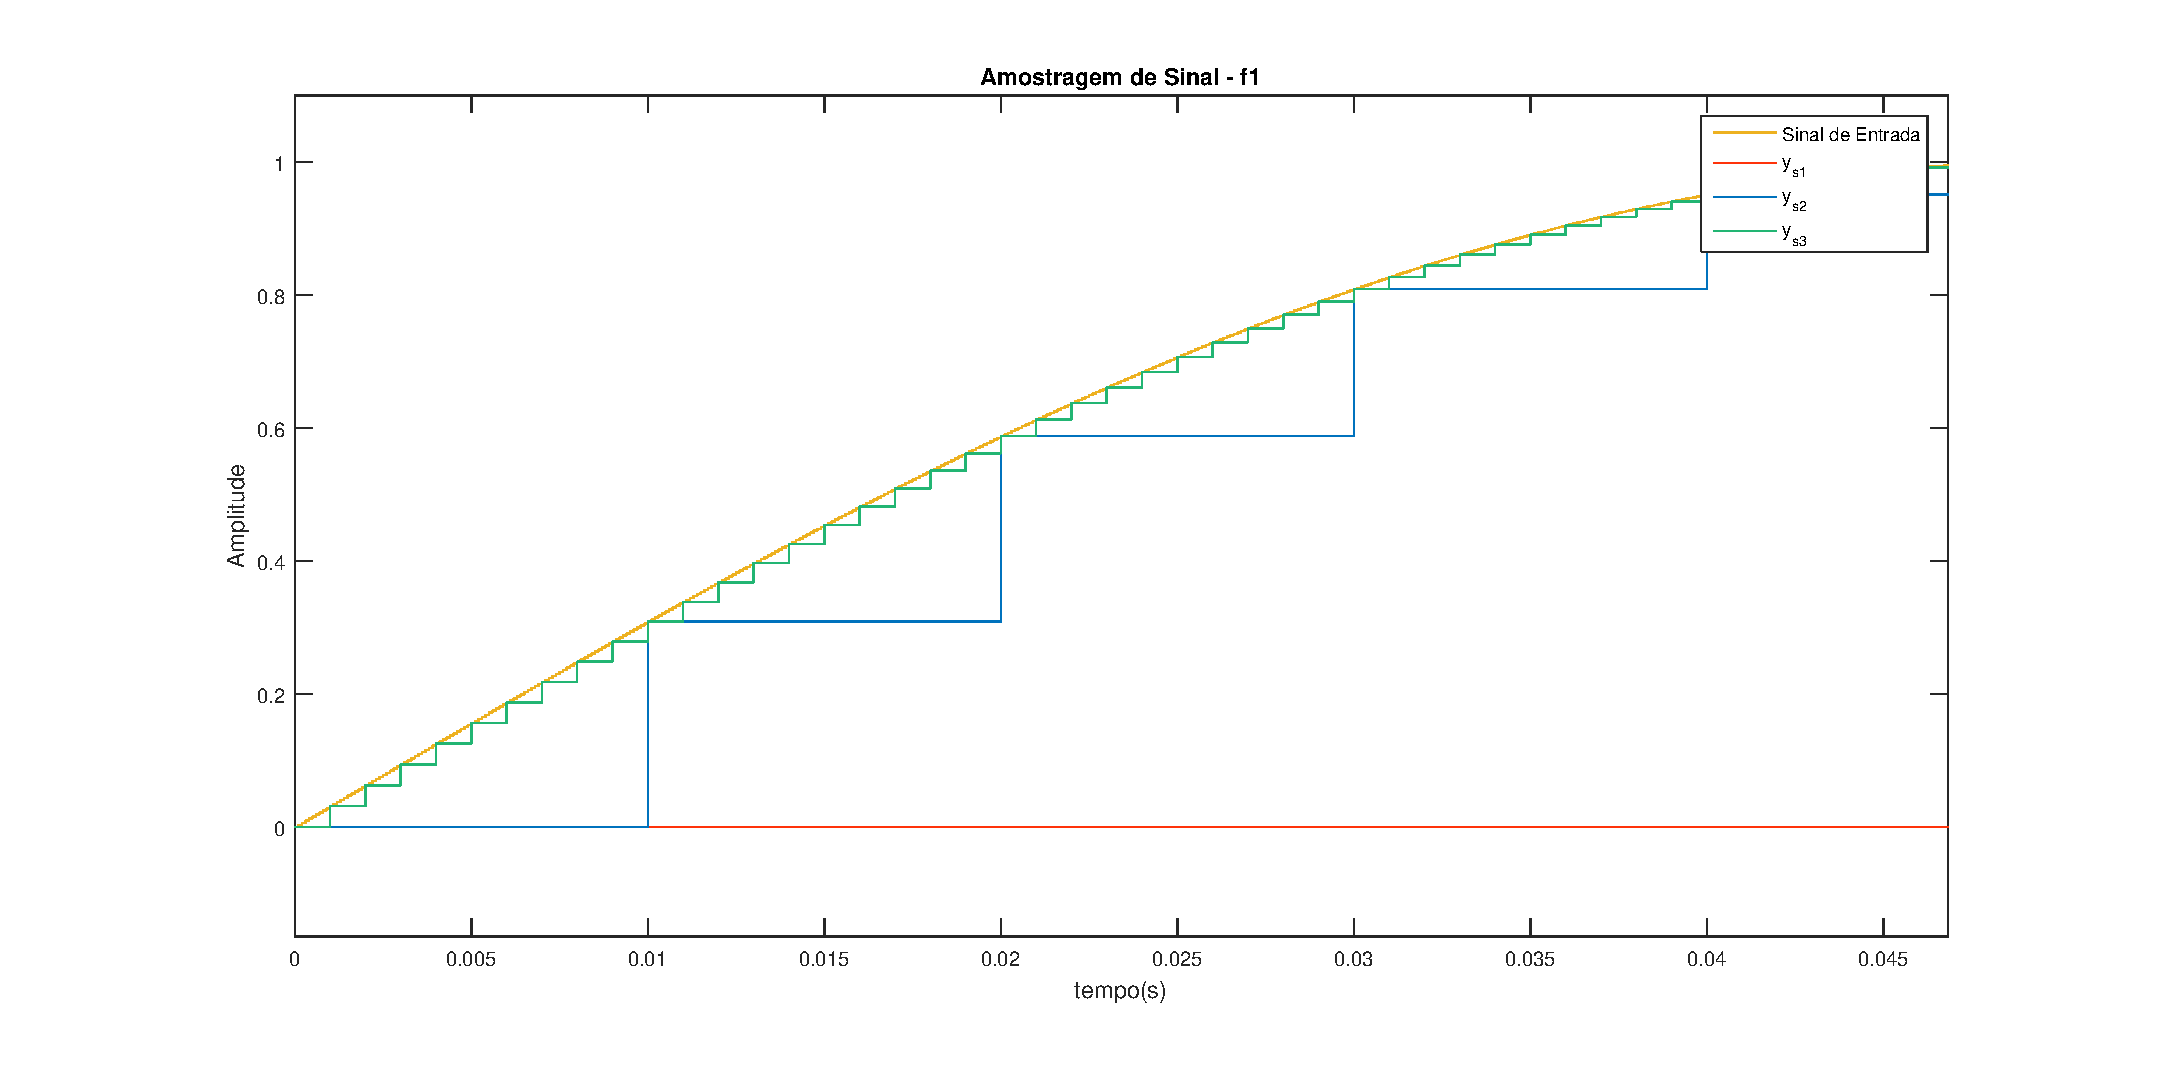
\includegraphics[scale = .45]{Imagens/pratica4_5.eps}
	\caption{Diagrama de blocos da prática 4.}
	\label{fig:pr4_esquema}
	\end{figure}
	
	\begin{figure}[!th]
		\centering
		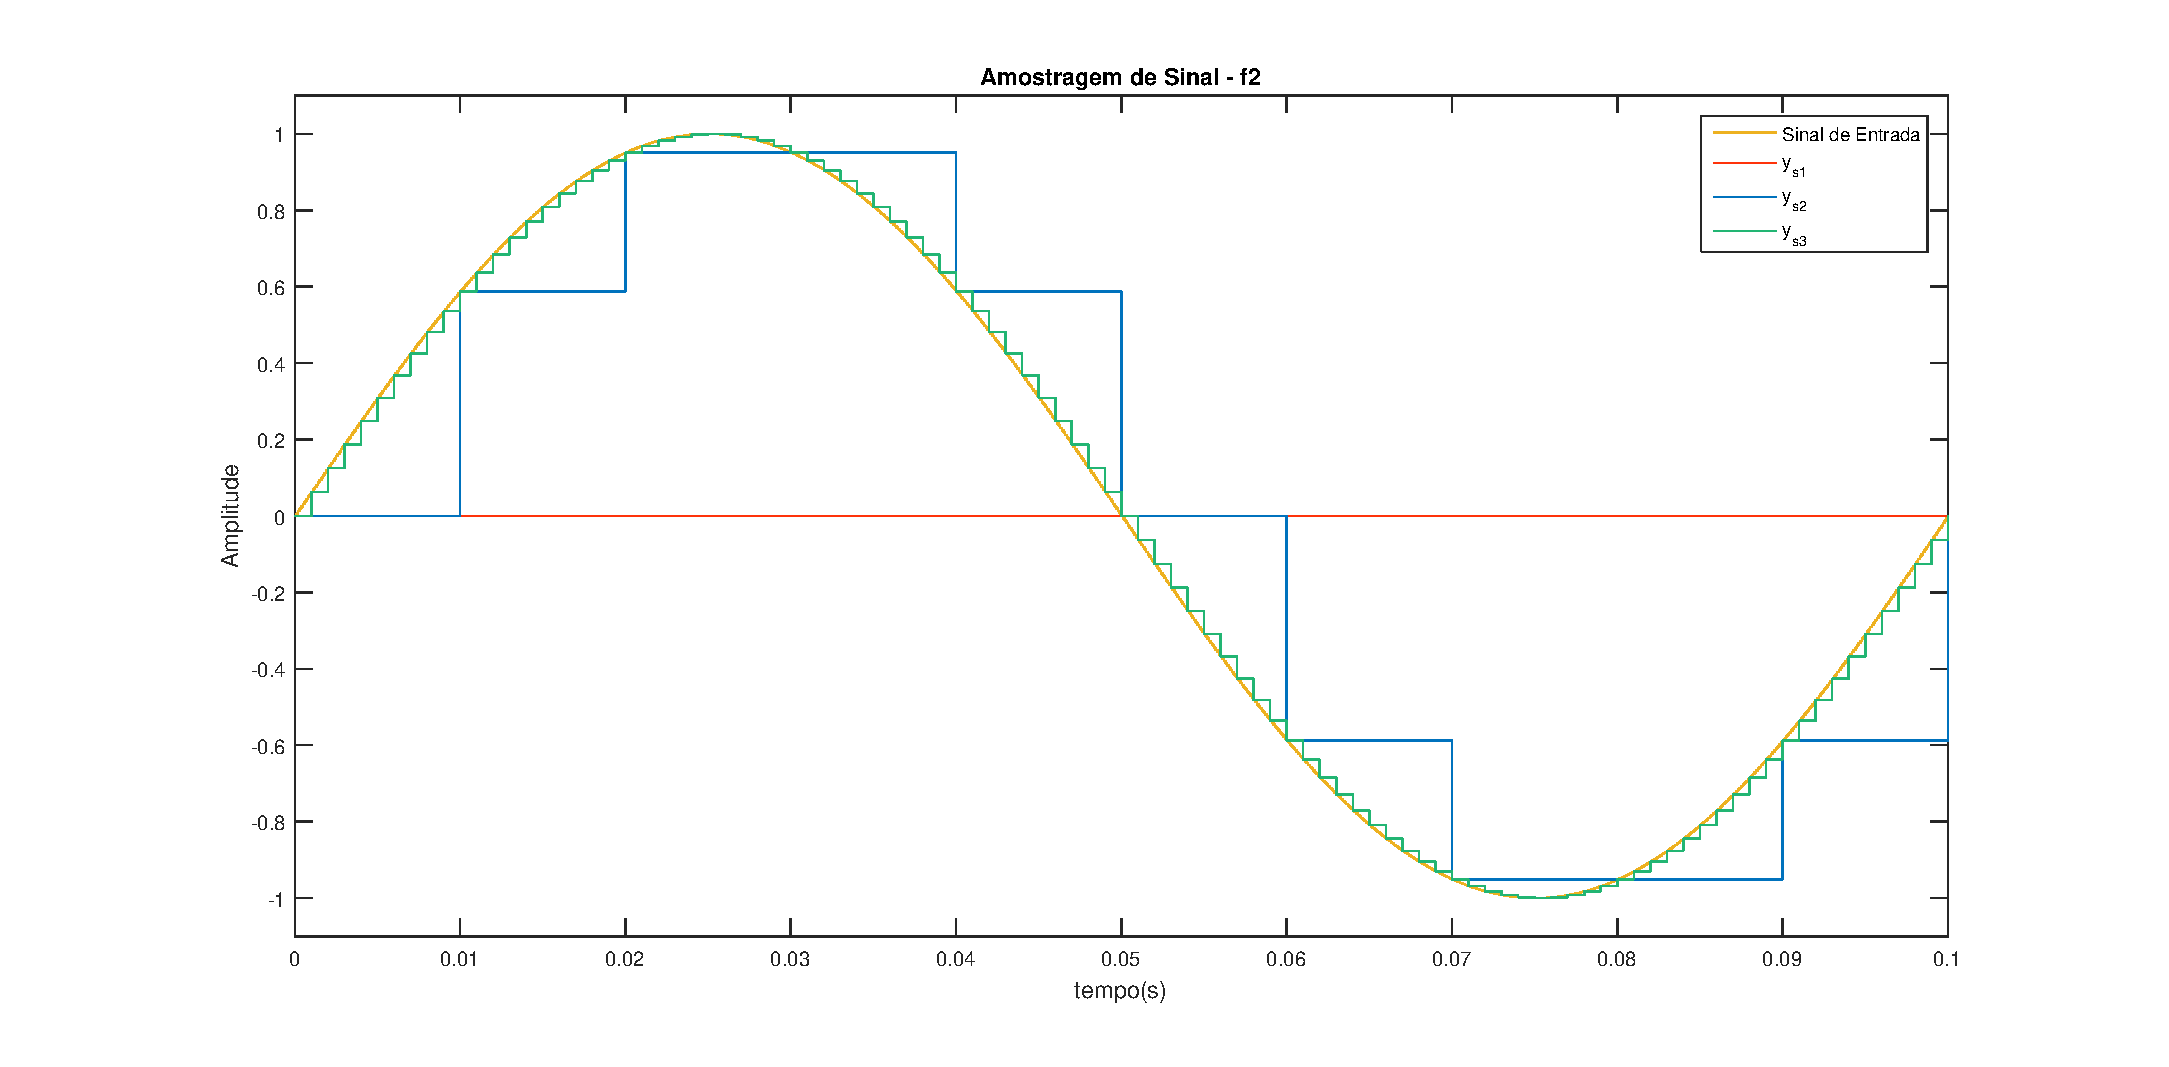
\includegraphics[scale = .45]{Imagens/pratica4_6.eps}
		\caption{Diagrama de blocos da prática 4.}
		\label{fig:pr4_esquema}
		\end{figure}

%---------- Quinta Prática  ----------
\chapter{Controlador PID}
\section{Objetivos}

\section{Fundamentação Teórica}

\section{Procedimentos}
\subsection{Exercício 1}
Considere um sistema em malha fechada com PID T(z) sendo:

\begin{figure}[H]
	\centering
	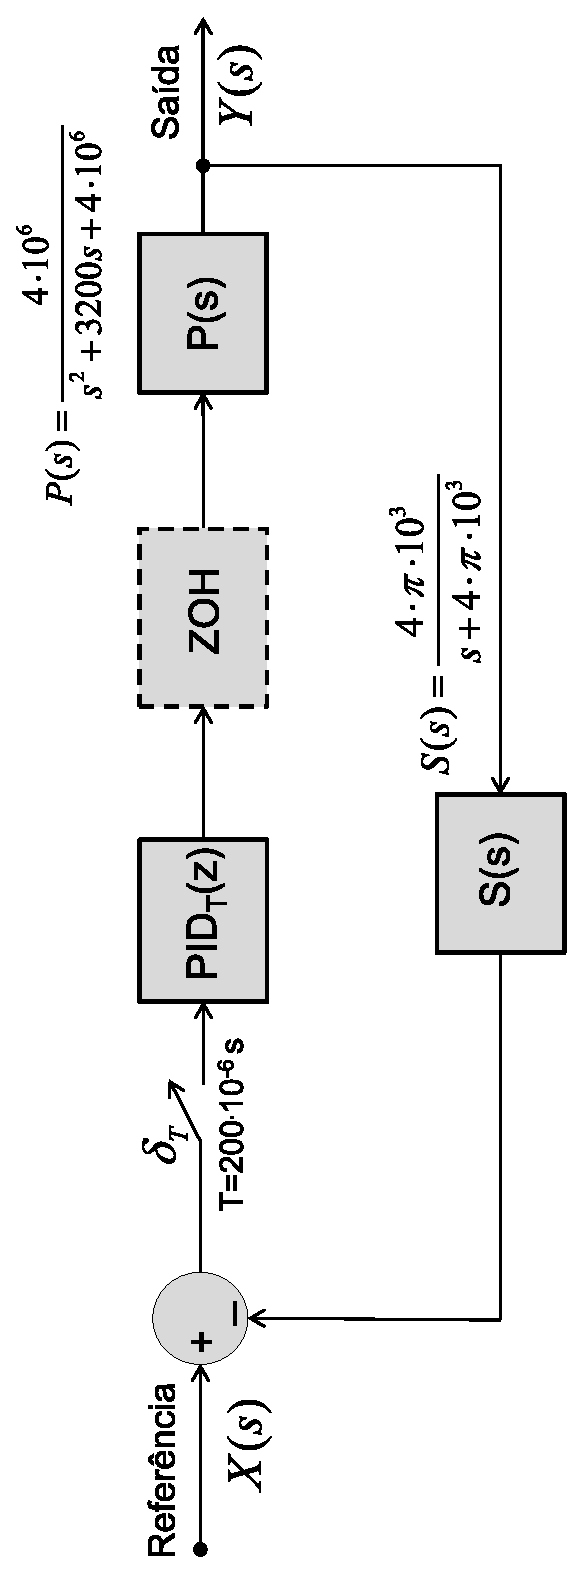
\includegraphics[scale = .5, angle =-90]{Imagens/PID.eps}
	\caption{Sistema - Exercício 1}
	\label{fig:ExercicioPID}
\end{figure}

Utilize simulações computacionais (Simulink\textregistered) para projetar ganhos para o controlador PID considerando a entrada um degrau unitário.

\subsection{Exercício 2}

Obtenha a função de transferência do PID de tempo discreto utilizando o método de discretização Forward para a parcela integral e considere Kp, Ki, e Kd como ganhos paralelos do controlador PID.

\subsubsection{Repita o Exercício 1 para esta função de transferência comparando os resultados de simulação de ambos os casos para os mesmos ganhos.}

\subsubsection{Inclua saturação na ação de controle em 150\% da referência e analise o comportamento do sistema de controle}

\subsection{Exercício 3}
Considerando o sistema descrito no exercício 2, desenvolva um script em Matlab para implementar o PID com os seguintes parâmetros.

\begin{itemize}
	\item Sinal de referência:
	Onda quadrada
	Amplitude $40~V_{pp}$
	Offset $0~V$
	Período $10ms$
	\item Controlador:
	PID ‘Digital’ (equação de diferenças)
	Saturação do PID (Sat = $0.98~V_{cc}$)
	\item Atuador: sinal PWM
	Resolução 8 bits (2n divisões)
	$V_{cc}=40~V$
	\item Ruído:
	Randômico
	Amplitude 2\% da saída
	\item Conversor A/D:
	Resolução 10 bits (2n níveis)
	Vin=0-5V
	T=200.10-6 s
	\item Planta
	$P(s)=\frac{4 \cdot 10^{6}}{s^{2}+3200s+4 \cdot 10^{6}}$
	\item Sensor
	$S(s)=\frac{4 \cdot \pi \cdot 10^{3}}{s + 4 \cdot \pi \cdot 10^{3}}$
\end{itemize}


\section{Resultados e discursões}

\subsection{Exercício 1}
	A partir do diagrama da Figura \ref{fig:ExercicioPID}, monta-se o circuito no Simulink\textregistered. A Figura \ref{fig:Exercicio1_PID_SimulinkII} apresenta o dado circuito implementado.

	\begin{figure}[H]
		\centering
		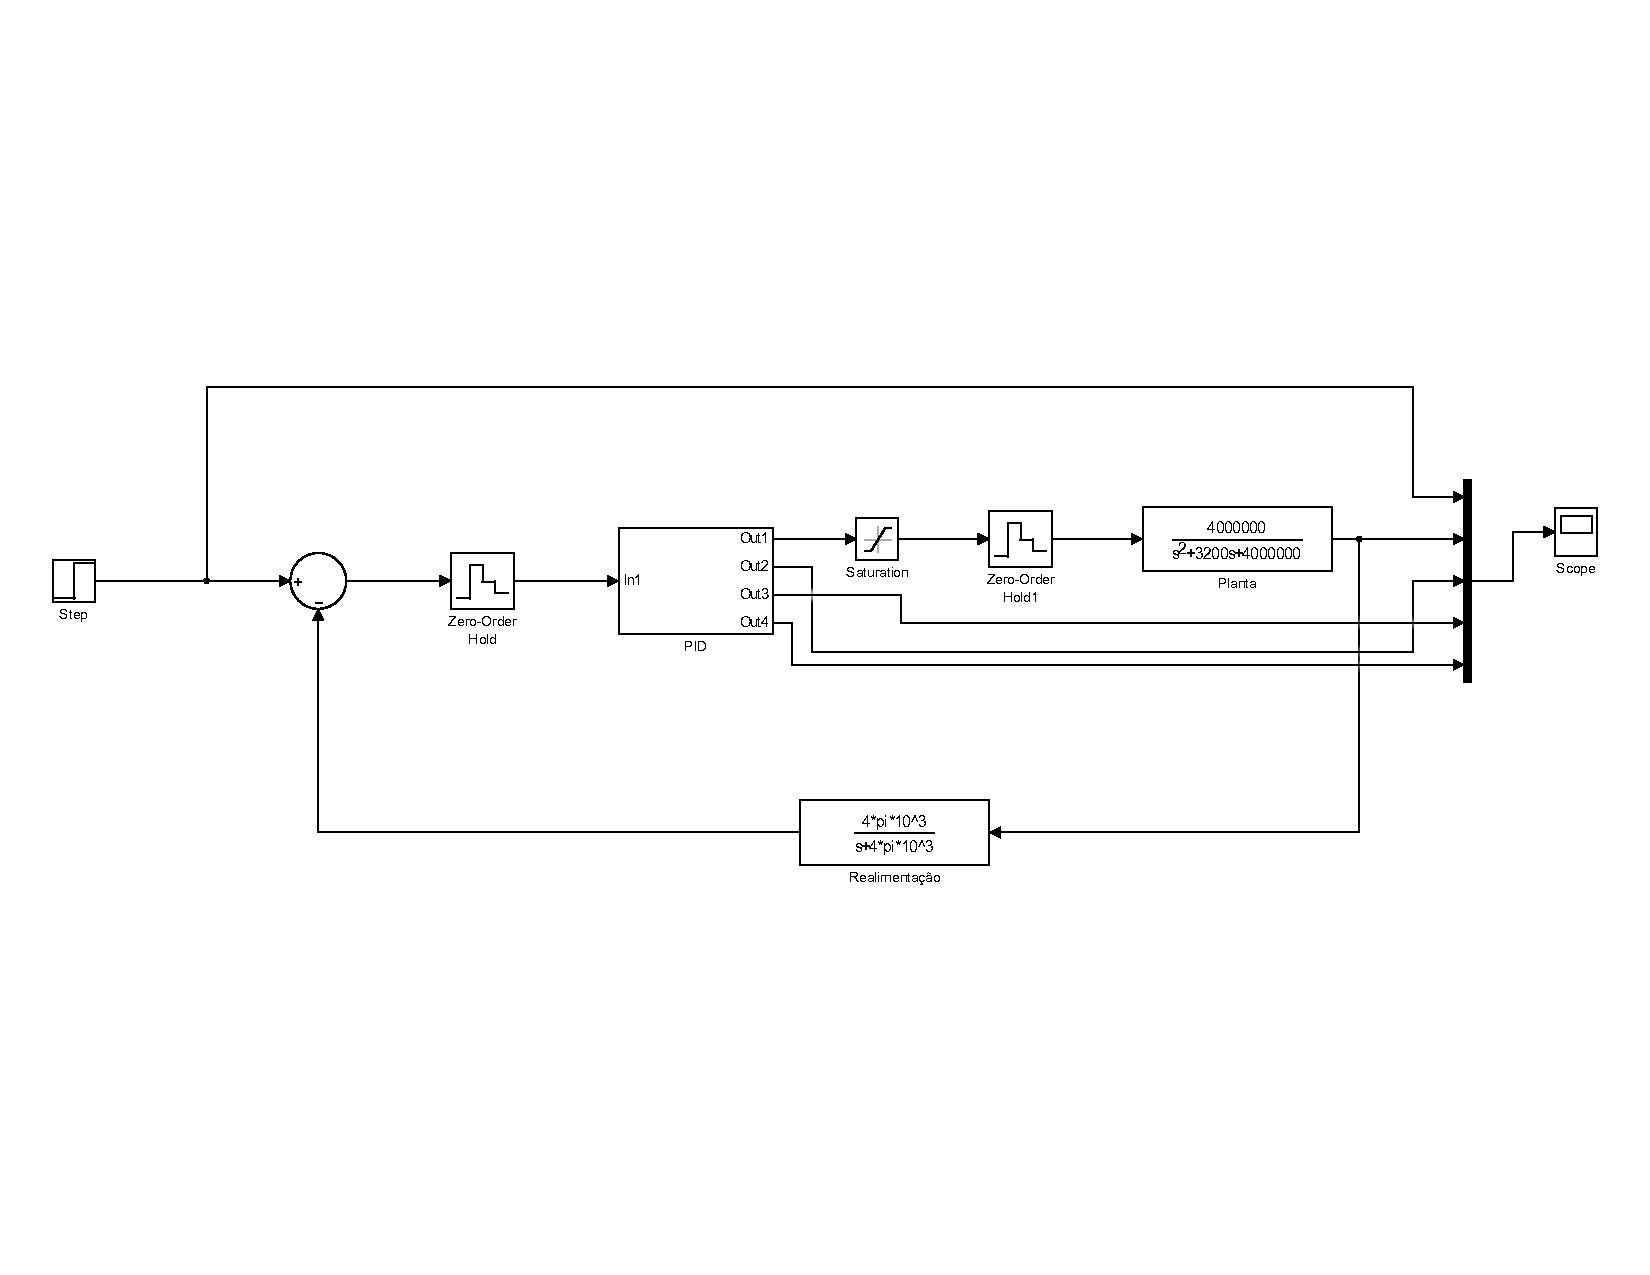
\includegraphics[scale = .4]{Imagens/Exercicio1_PID_SimulinkII.pdf}
		\caption{Diagrama de Blocos Exercício 1}
		\label{fig:Exercicio1_PID_SimulinkII}
	\end{figure}
	
	 A Figura \ref{fig:Exercicio1_PID_Simulink} está apresentado o circuito PID implementado. Os valores $K_P$, $K_D$ e $K_I$ são obtidos a partir dos método de projeto Ziegler-Nichols usando o procedimento 2. Ou seja foi obtido um ganho critico em malha fechada de modo que provoque um sinal de saída com oscilações constantes, e com base neste ganho e no período das oscilações constantes se defini os valores dos ganhos do PID.
	
	\begin{figure}[H]
		\centering
		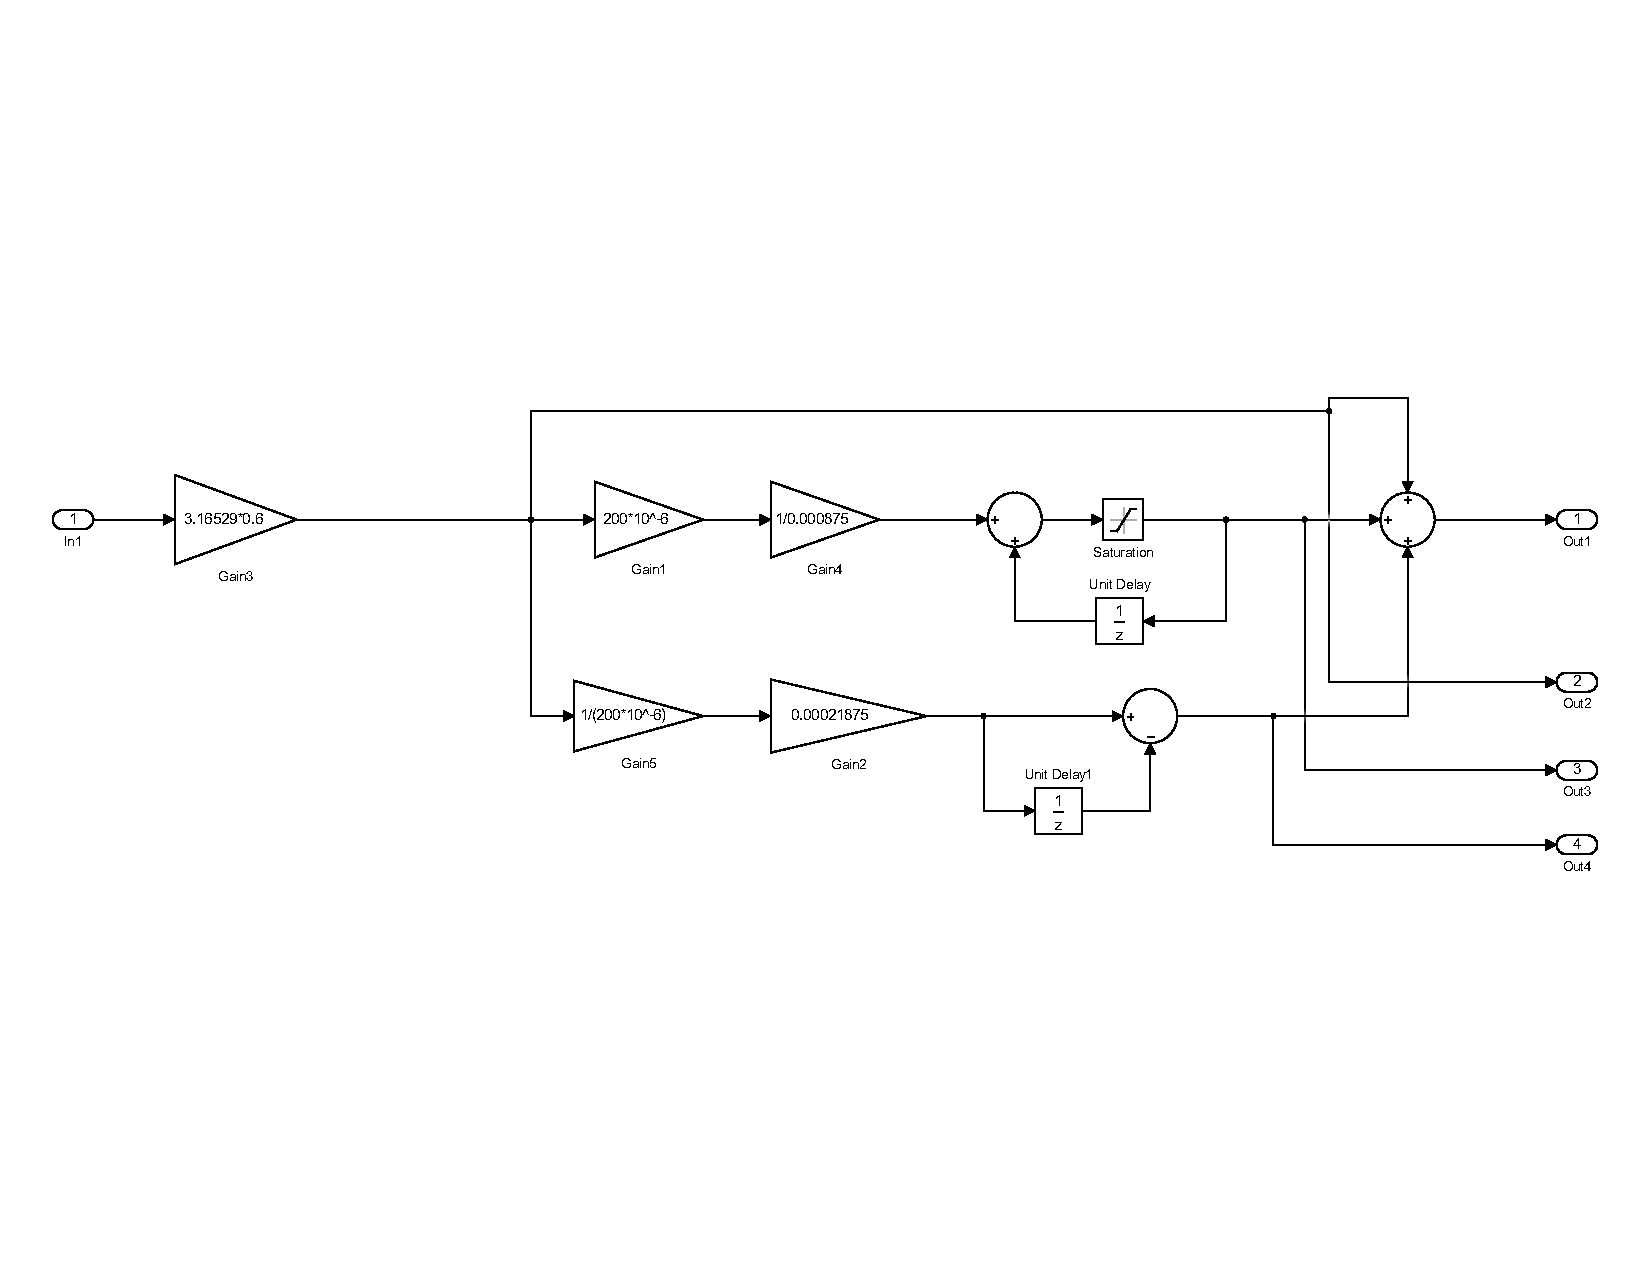
\includegraphics[scale = .4]{Imagens/Exercicio1_PID_Simulink.pdf}
		\caption{Diagrama de Blocos Exercício 1 - PID}
		\label{fig:Exercicio1_PID_Simulink}
	\end{figure}
	
\subsection{Exercício 2}
	Para a obtenção da função transferência do PID de tempo discreto usando o método de discretização \emph{Forward} se parte da equação básica do PID, definida pela Equação \ref{PIDEmTempo}.
	
	\begin{equation}
		u(t) = K \left( e(t) + \frac{1}{T_{i}} \int_0^t e(t) dt + T_d \frac{d}{dt} e(t) \right) 
		\label{PIDEmTempo}
	\end{equation}
	
	Seguindo a discretização, tornando $u_k = u(k)$ é possível aproximar a parcela de erro pela Equação \ref{erro}, a parcela integral pela Equação \ref{integral}, proveniente da discretização \emph{Forward}. E por fim a parcela derivativa pela Equação \ref{derivada}.
	
	\begin{equation}
		e(t) \rightarrow e_k
		\label{erro}
	\end{equation}
		
	\begin{equation}
		\int_0^t e(t) dt \rightarrow \sum_{i=0}^{k} e_i T
		\label{integral}
	\end{equation}
	
	\begin{equation}
		\frac{d}{dt} e(t) \rightarrow \frac{e_k - e_{k-1}}{T}
		\label{derivada}
	\end{equation}
	
	Logo pode-se definir a forma discreta do PID pela Equação \ref{PIDDiscreto}.
	 
	\begin{equation}
	u_k = K \left( e_k + \frac{T}{T_i} \sum_{i=0}^{k} (e_i) + \frac{T_d}{T}(e_k - e_{k-1})\right)
	\label{PIDDiscreto}
	\end{equation}
	
			

%---------- Sexta Prática  ----------
\chapter{Controlador Repetitivo}
\section{Objetivos}

\section{Fundamentação Teórica}

\section{Procedimentos}

\section{Resultados e discursões}

%---------- Sétima e oitava prática - 19/04/2016 ----------
\chapter{Transformada Z}
\section{Objetivos}

\section{Fundamentação Teórica}

\section{Procedimentos}

\section{Resultados e discursões}

\chapter{Transformada Z inversa}
\section{Objetivos}

\section{Fundamentação Teórica}

\section{Procedimentos}

\section{Resultados e discursões}

%---------- (Conclusão)--------
\chapter{Conclusão}


%---------- Referencias ----------
\bibliography{referencias}
%---------- Fim do documento ----------
\end{document}